\documentclass[11pt]{article}
\usepackage{url}
\usepackage{graphicx}

\usepackage{course}
\begin{document}
\ctitle{1}{Decision trees and k-Nearest Neighbors}{Oct. 29, 2020 at 11:59 pm}
\author{}
\date{}
\vspace{-1in}
\maketitle
\vspace{-0.75in}


\blfootnote{Parts of this assignment are adapted from course material by Andrea Danyluk (Williams), Tom Mitchell, Matt Gormley and Maria-Florina Balcan (CMU), Stuart Russell (UC Berkeley), Carlos Guestrin (UW), Dan Roth (UPenn) and Jessica Wu (Harvey Mudd). }




\section*{Submission instructions}
\begin{itemize}
\item 
Submit your solutions electronically on the course Gradescope site as PDF files.
\item Please package your code (.py) for Problem 5 and submit it to CCLE.
\item If you plan to typeset your solutions, please use the LaTeX solution template. If you must submit scanned handwritten solutions, please use a black pen on blank white paper and a high-quality scanner app.
\end{itemize}

\clearpage

\section{Splitting Heuristic for Decision Trees \problemworth{20}}
Recall that the ID3 algorithm iteratively grows a decision tree from the root downwards. On each iteration, the algorithm replaces one leaf node with an internal node that splits the data based on one decision attribute (or feature). In particular, the ID3 algorithm chooses the split that reduces the entropy the most, but there are other choices. For example, since our goal in the end is to have the lowest error, why not instead choose the split that reduces error the most? In this problem, we will explore one reason why reducing entropy is a better criterion.

Consider the following simple setting. Let us suppose each example is described by $n$ boolean features: $X = \langle X_1, \ldots, X_n \rangle$, where $X_i \in \{0, 1\}$, and where $n \geq 4$. Furthermore, the target function to be learned is $f : X \rightarrow Y$, where $Y = X_1 \vee X_2 \vee X_3$. That is, $Y = 1$ if $X_1 = 1$ or $X_2 = 1$ or $X_3 = 1$, and $Y = 0$ otherwise. Suppose that your training data contains all of the $2^n$ possible examples, each labeled by $f$. For example, when $n = 4$, the data set would be
\begin{table}[H]
\centering
\begin{tabular}{cccc|c}
$X_1$ & $X_2$ & $X_3$ & $X_4$ & $Y$\\ \hline
0 & 0 & 0 & 0 & 0\\
1 & 0 & 0 & 0 & 1\\
0 & 1 & 0 & 0 & 1\\
1 & 1 & 0 & 0 & 1\\
0 & 0 & 1 & 0 & 1\\
1 & 0 & 1 & 0 & 1\\
0 & 1 & 1 & 0 & 1\\
1 & 1 & 1 & 0 & 1\\
\end{tabular}
\quad \quad \quad \quad
\begin{tabular}{cccc|c}
$X_1$ & $X_2$ & $X_3$ & $X_4$ & $Y$\\ \hline
0 & 0 & 0 & 1 & 0\\
1 & 0 & 0 & 1 & 1\\
0 & 1 & 0 & 1 & 1\\
1 & 1 & 0 & 1 & 1\\
0 & 0 & 1 & 1 & 1\\
1 & 0 & 1 & 1 & 1\\
0 & 1 & 1 & 1 & 1\\
1 & 1 & 1 & 1 & 1\\
\end{tabular}
\end{table}

\begin{enumerate}
\item \itemworth{5} How many mistakes does the best $1$-leaf decision tree make over the $2^n$ training examples? (The $1$-leaf decision tree does not split the data even once. Make sure you answer for the general case when $n \geq 4$.)

\solution{}

\item \itemworth{5} Is there a split that reduces the number of mistakes by at least one? (That is, is there a decision tree with $1$ internal node with fewer mistakes than your answer to part (a)?) Why or why not?

\solution{}

\item \itemworth{5} What is the entropy of the output label $Y$ for the $1$-leaf decision tree (no splits at all)?

\solution{}

\item \itemworth{5} Is there a split that reduces the entropy of the output $Y$ by a non-zero amount? If so, what is it, and what is the resulting conditional entropy of $Y$ given this split?

\solution{}

\end{enumerate}

\ifsoln 
\else
\clearpage
\fi

\section{Entropy and Information \problemworth{5}}
The entropy of a Bernoulli (Boolean 0/1) random variable $X$ with $p(X = 1) = q$ is given by
\begin{equation*}
B(q) = - q \log q - (1 - q) \log(1 - q).
\end{equation*}
Suppose that a set $S$ of examples contains $p$ positive examples and $n$ negative examples. The entropy of $S$ is defined as $H(S) = B\left(\frac{p}{p+n}\right)$.
\begin{enumerate}
\item \itemworth{5} Based on an attribute $X_j$, we split our examples into $k$ disjoint subsets $S_k$, with $p_k$ positive and $n_k$ negative examples in each. If the ratio $\tfrac{p_k}{p_k + n_k}$ is the same for all $k$, show that the information gain of this attribute is 0.

\solution{}
\end{enumerate}

% \newpage
\section{k-Nearest Neighbors and Cross-validation \problemworth{10}}
In the following questions you will consider a $k$-nearest neighbor classifier using Euclidean
distance metric on a binary classification task. 
We assign the class of the test point to be the
class of the majority of the $k$ nearest neighbors. 
Note that a point can be its own neighbor.
\begin{figure}[h]
    \centering
    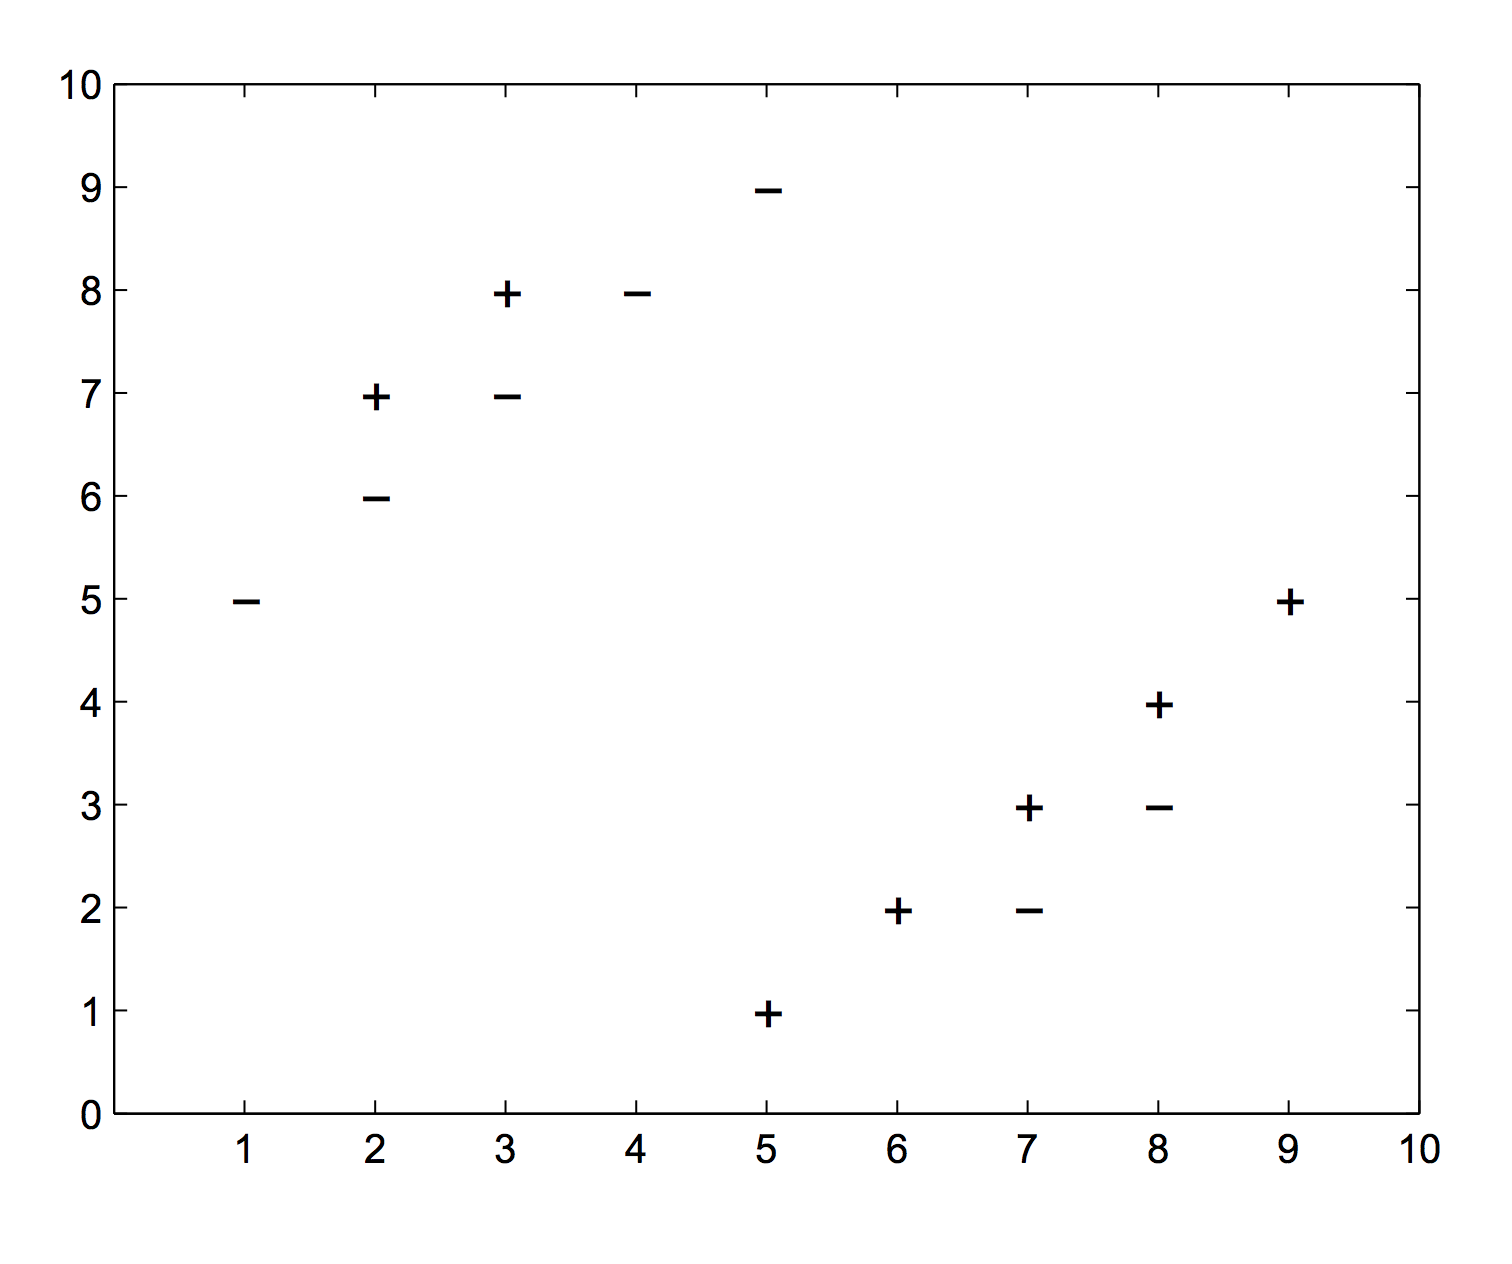
\includegraphics[scale=0.45]{knn_figure.png}
    \caption{Dataset for KNN binary classification task.}
    \label{fig:knn}
\end{figure}

\begin{enumerate}

    \item \itemworth{2.5} What will be the label of point (7,3) in Fig \ref{fig:knn} using K-NN algorithm with majority voting when $K$=3?

\\
\solution{}

    \item \itemworth{2.5} What value of $k$ minimizes the training set error for this dataset? What is
the resulting training error?

\solution{}

    \item \itemworth{2.5} Why might using too large values $k$ be bad in this dataset? Why might too
small values of k also be bad?

\solution{}

    \item \itemworth{2.5} What value of $k$ minimizes leave-one-out cross-validation error for this
dataset? What is the resulting error?

\solution{}
\end{enumerate}
\section{Decision Tree \problemworth{15}}
In a binary classification problem, there are $4000$ examples in the  class with label $1$ and $8000$ examples in the class with label $0$.     
Recall that the information gain for target label $Y$ and feature $X$ is defined as $Gain = H [Y] - H [Y |X ]$, where $H [Y ] = - E[\log_2 P (Y )]$ is the entropy.


\begin{enumerate}
\item\itemworth{2}  What is the entropy of the class variable $Y$?

\solution{}
% \newpage

\item \itemworth{5} Let's consider a binary feature $A$ for this problem. In the negative class (with label $0$), the number of instances that have $A=1$ and $A=0$ respectively: $(4000,4000)$. In the positive class (with label $1$), these numbers are: $(4000, 0)$. Write down conditional entropy and information gain of $A$ relative to $Y$?\\

\solution{}
        % \newpage
\item\itemworth{5} 
Let's consider another binary feature $B$. In the negative class (with label $0$) , the number of instances that have $B=0$ and $B=1$ respectively are: $(6000,2000)$. In the positive class (with label $1$), these numbers are: $(3000,1000)$. Write down conditional entropy and information gain of $B$ relative to $Y$?\\
\solution{}
% \newpage

\item\itemworth{3} 
Using information gain, which attribute will the ID3 decision tree learning algorithm choose at first?

\solution{}

\end{enumerate}


\newpage
\section{Programming exercise : Applying decision trees and k-nearest neighbors \problemworth{50}}

\ifsoln
\else

\section*{Introduction\footnote{This assignment is adapted from the UCI Machine learning repository, available at \url{https://archive.ics.uci.edu/ml/datasets/adult}.}}

This data was extracted from the 1994 Census bureau database by Ronny Kohavi and Barry Becker. For computational reasons, we have already extracted a relatively clean subset of the data for this HW. The prediction task is to determine whether a person makes over \$50K a year.

In this problem, we ask you to complete the analysis of what sorts of people were likely to earn more than \$50K a year. In particular, we ask you to apply the tools of machine learning to predict which individuals are more likely to have high income. 


\section*{Starter Files}

\vspace{-\baselineskip}
\rule{\textwidth}{1pt}
code and data
\begin{itemize}[nolistsep]
\item Code: \href{https://colab.research.google.com/drive/1_O5QwkZ33fnYbW3zwSnKjeVYkeoEtIeD?usp=sharing}{Fall2020-CS146-HW1.ipynb}\item Data: \href{https://drive.google.com/drive/folders/1xjZlT1TzoJ79Hd48fdjI1-gk7hnNOwTz?usp=sharing}{nutil.py and adult\_subsample.csv} 


\end{itemize}
documentation
\begin{itemize}[nolistsep]
\item Decision Tree Classifier: \\{\footnotesize \url{http://scikit-learn.org/stable/modules/generated/sklearn.tree.DecisionTreeClassifier.html}}
\item K-Nearest Neighbor Classifier: \\{\footnotesize \url{http://scikit-learn.org/stable/modules/generated/sklearn.neighbors.KNeighborsClassifier.html}} 
\item Cross-Validation: \\{\footnotesize \url{https://scikit-learn.org/stable/modules/generated/sklearn.model_selection.StratifiedShuffleSplit.html}}
\item Metrics: \\ {\footnotesize \url{http://scikit-learn.org/stable/modules/generated/sklearn.metrics.accuracy_score.html}, \\
\url{https://scikit-learn.org/stable/modules/generated/sklearn.metrics.f1_score.html?highlight=f1%20score#sklearn.metrics.f1_score}} 
\item Data Preprocessing: \\{\footnotesize \url{https://scikit-learn.org/stable/modules/generated/sklearn.preprocessing.StandardScaler.html?highlight=standardscaler#sklearn.preprocessing.StandardScaler}}
\end{itemize}
\vspace{-\baselineskip}
\rule{\textwidth}{1pt}


Note that any portions of the code that you must modify have been indicated with \verb|TODO|. Do not change any code outside of these blocks.
\fi

To work on this HW: you need to download two files (i) nutil.py (ii) adult\_subsample.csv from  \href{https://drive.google.com/drive/folders/1xjZlT1TzoJ79Hd48fdjI1-gk7hnNOwTz?usp=sharing}{here}. Then copy/upload them to you own Google drive. 

\ifsoln
\else
\clearpage
\fi

Next, for all the coding, please refer to the following colab notebook  
\href{https://colab.research.google.com/drive/1_O5QwkZ33fnYbW3zwSnKjeVYkeoEtIeD?usp=sharing}{Fall2020-CS146-HW1.ipynb}. 

\textbf{Before executing or writing down any code, please make a copy of the notebook and save it to your own google drive by clicking the “File” $\rightarrow$ “Save a copy in Drive”.} 

\begin{minipage}[c]{.5\textwidth}
%\begin{figure}[H]
\centering
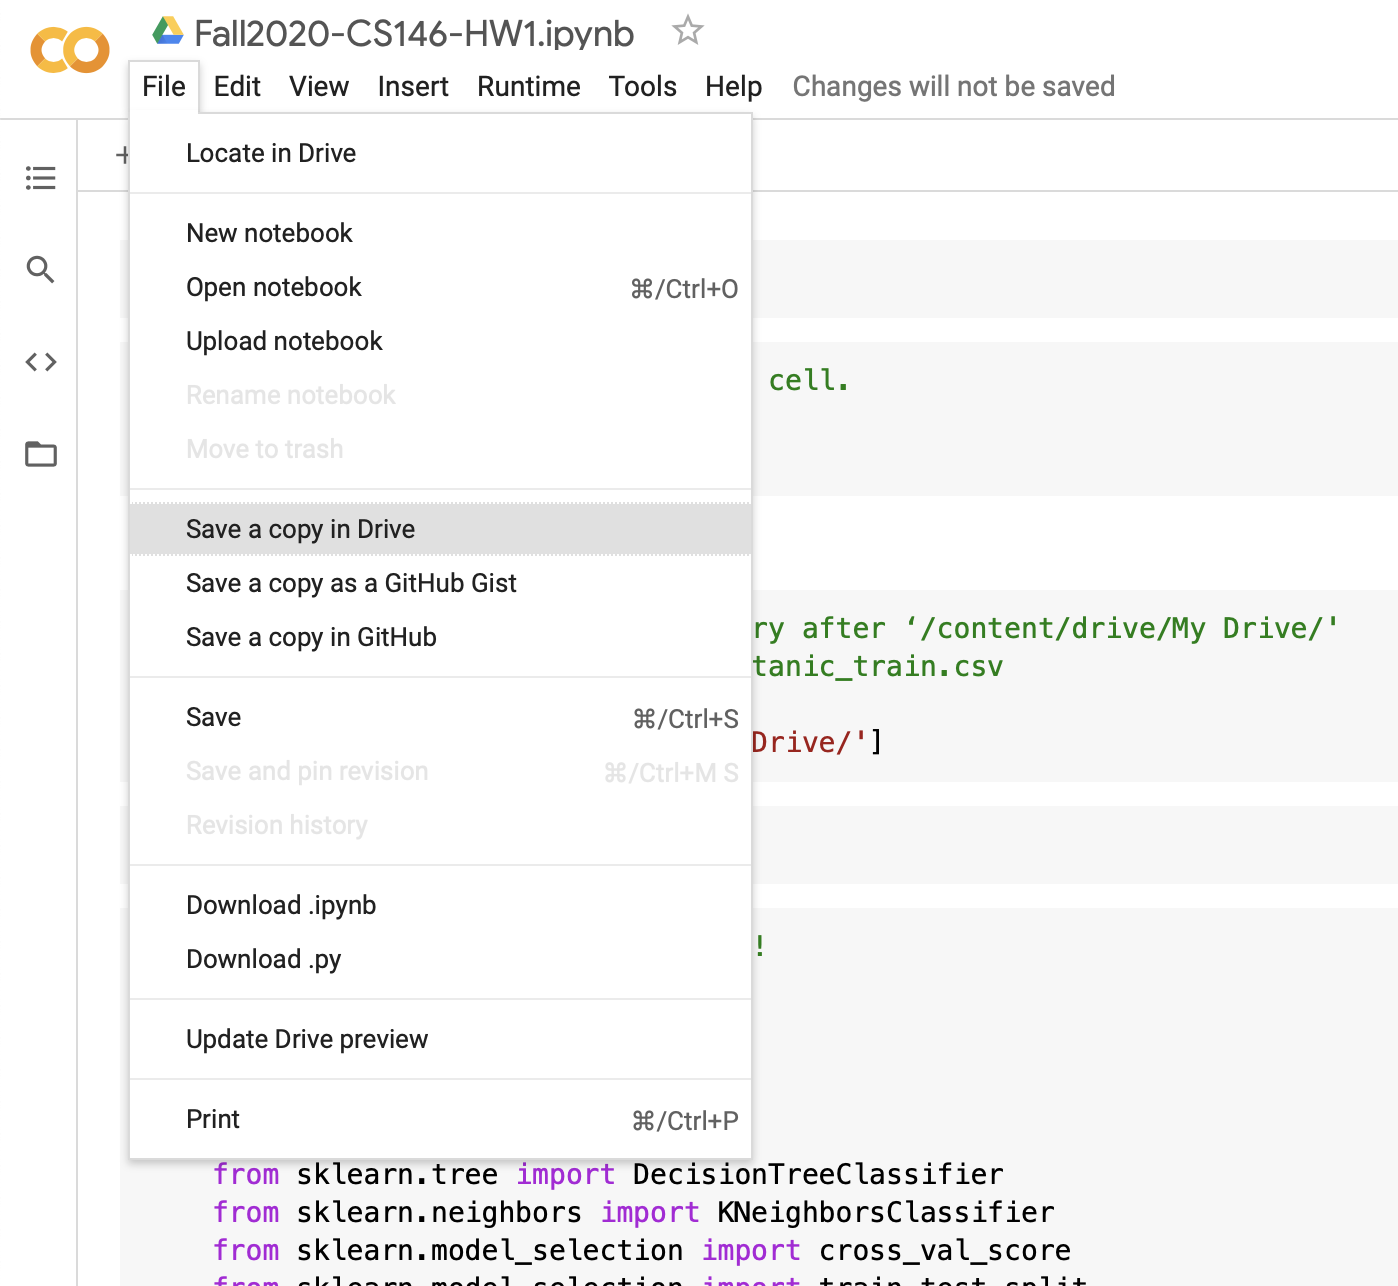
\includegraphics[scale=0.5]{save-colab-to-drive.png}
%\end{figure}
\end{minipage}%
\begin{minipage}[c]{.45\textwidth}
\end{minipage}%


You will then be prompted to log into your google account. Please make sure all the work you implement is done on your own saved copy. You won’t to able to make changes on the the original notebook shared for the entire class. Running the first two cells will further mount your own google drive so that your copy of the Colab notebook will have access to the two files (nutil.py and adult\_subsample.csv) you’ve just uploaded.

The notebook has marked blocks where you need to code. \\
\\
 $### ========= TODO  : START ========= ### $
 
 $### ========= TODO :  END   ========== ###$
\\

\ifsoln
\else
\clearpage
\fi

\section*{Submission instructions for programming problems}
\begin{itemize}
\item Please export the notebook to a \verb|.py| file by clicking the “File” $\rightarrow$ “Download.py” and upload to CCLE.} 

Your code should be commented appropriately. The most important things:
\vspace{-\parskip}
\begin{itemize}[nosep]
\item Your name and the assignment number should be at the top of each file.
\item Each class and method should have an appropriate doctsring.
\item If anything is complicated, it should include some comments.
\end{itemize}
\vspace{-\parskip}
There are many possible ways to approach the programming portion of this assignment, which makes code style and comments very important so that staff can understand what you did. For this reason, you will lose points for poorly commented or poorly organized code.
\end{itemize}

\begin{itemize}
\item Please submit all the plots and the rest of the solutions (other than codes) to Gradescope
\end{itemize}



For the questions please read below.

\subsection{Visualization \problemworth{5}}
One of the first things to do before trying any formal machine learning technique is to dive into the data. This can include looking for funny values in the data, looking for outliers, looking at the range of feature values, what features seem important, etc.

Note: We have already converted all the categorical features to numerical ones. The target column is the last one: "$>$50k", where 1 and 0 indicate $>$50k or $\le$ 50k respectively. The feature "fnlwgt" describes the number of people the census believes the entry represents. All the other feature names should be self-explanatory. If you want to learn more about this data please click  \href{https://archive.ics.uci.edu/ml/datasets/adult}{here}

\begin{enumerate}
\item \itemworth{5} Make histograms for each feature, separating the examples by class (e.g. income greater than 50k or smaller than or equal to 50k). This should produce fourteen plots, one for each feature, and each plot should have two overlapping histograms, with the color of the histogram indicating the class. For each feature, what trends do you observe in the data? (Please only describe the general trend. No need for more than two sentences per feature) 

\solution{}

\end{enumerate}

\ifsolution{\newpage}
\subsection{Evaluation \problemworth{45}}

Now, let's use \verb|scikit-learn| to train a \verb|DecisionTreeClassifier| and \verb|KNeighborsClassifier| on the data.

Using the predictive capabilities of the \verb|scikit-learn| package is very simple. In fact, it can be carried out in three simple steps: initializing the model, fitting it to the training data, and predicting new values.\footnote{Note that almost all of the model techniques in \verb|scikit-learn| share a few common named functions, once they are initialized. You can always find out more about them in the documentation for each model. These are \verb|some-model-name.fit(...)|, \verb|some-model-name.predict(...)|, and \verb|some-model-name.score(...)|.}


\begin{enumerate}[resume]

\item \itemworth{0} Before trying out any classifier, it is often useful to establish a \emph{baseline}. We have implemented one simple baseline classifier, \verb|MajorityVoteClassifier|, that always predicts the majority class from the training set. Read through the \verb|MajorityVoteClassifier| and its usage and make sure you understand how it works.

Your goal is to implement and evaluate another baseline classifier, \verb|RandomClassifier|, that predicts a target class according to the distribution of classes in the training data set. For example, if 85\% of the examples in the training set have \verb|>50k = 0| and 15\% have \verb|>50k = 1|, then, when applied to a test set, \verb|RandomClassifier| should randomly predict 85\% of the examples as \verb|>50k = 0| and 15\% as \verb|>50k = 1|.

Implement the missing portions of \verb|RandomClassifier| according to the provided specifications. Then train your \verb|RandomClassifier| on the entire training data set, and evaluate its training error. If you implemented everything correctly, you should have an error of {\color {red} {$0.374$.} }

\item \itemworth{10} Now that we have a baseline, train and evaluate a \verb|DecisionTreeClassifier| (using the class from \verb|scikit-learn| and referring to the documentation as needed). Make sure you initialize your classifier with the appropriate parameters; in particular, use the `entropy' criterion discussed in class. What is the training error of this classifier?
\solution{}

\item \itemworth{5} Similar to the previous question, train and evaluate a \verb|KNeighborsClassifier| (using the class from \verb|scikit-learn| and referring to the documentation as needed). Use $k$=3, 5 and 7 as the number of neighbors and report the training error of this classifier.
\solution{}

\item \itemworth{10} So far, we have looked only at training error, but as we learned in class, training error is a poor metric for evaluating classifiers. Let's use cross-validation instead.

Implement the missing portions of \verb|error(...)| according to the provided specifications. You may find it helpful to use \verb|StratifiedShuffleSplit(...)| from \verb|scikit-learn|. To ensure that we always get the same splits across different runs (and thus can compare the classifier results), set the \verb|random_state| parameter to be the same (e.g., 0).


Next, use your \verb|error(...)| function to evaluate the training error and (cross-validation) test error and test micro averaged F1 Score (If you dont know what is F1, please click \href{https://scikit-learn.org/stable/modules/generated/sklearn.metrics.f1_score.html?highlight=f1\%20score#sklearn.metrics.f1_score}{here}) of each of your four models (for the \verb|KNeighborsClassifier|, use $k$=5). To do this, generate a random $80/20$ split of the training data, train each model on the $80\%$ fraction, evaluate the error on either the $80\%$ or the $20\%$ fraction, and repeat this $100$ times to get an average result. What are the average training and test error of each of your classifiers on the adult\_subsample data set?

\solution{}


\item \itemworth{5} One way to find out the best value of $k$ for \verb|KNeighborsClassifier| is $n$-fold cross validation.
Find out the best value of $k$ using 10-fold cross validation. You may find the \verb|cross_val_score(...)| from \verb|scikit-learn| helpful. Run 10-fold cross validation for all odd numbers ranging from 1 to 50 as the number of neighbors.
Then plot the validation error against the number of neighbors, $k$.
Include this plot in your writeup, and provide a 1-2 sentence description of your observations. What is the best value of $k$?

\solution{}

\item \itemworth{5} One problem with decision trees is that they can \emph{overfit} to training data, yielding complex classifiers that do not generalize well to new data. Let's see whether this is the case.

One way to prevent decision trees from overfitting is to limit their depth. Repeat your cross-validation experiments but for increasing depth limits, specifically, $1,2,\ldots,20$. Then plot the average training error and test error against the depth limit. 
Include this plot in your writeup, making sure to label all axes and include a legend for your classifiers. What is the best depth limit to use for this data? Do you see overfitting? Justify your answers using the plot.

\solution{}

\item \itemworth{5} Another useful tool for evaluating classifiers is \emph{learning curves}, which show how classifier performance (e.g. error) relates to experience (e.g. amount of training data).
For this experiment, first generate a random 90/10 split of the training data and do the following experiments considering the 90\% fraction as training and 10\% for testing. 

Run experiments for the decision tree and k-nearest neighbors classifier with the best depth limit and $k$ value you found above.
This time, vary the amount of training data by starting with splits of $0.10$ ($10\%$ of the data from 90\% fraction) and working up to full size $1.00$ ($100\%$ of the data from 90\% fraction) in increments of $0.10$. Then plot the decision tree and k-nearest neighbors training and test error against the amount of training data. 
Include this plot in your writeup, and provide a 1-2 sentence description of your observations.

\solution{}

\item \itemworth{5} Pre-process the data by standardizing it. See the sklearn.preprocessing.StandardScaler package for details. After performing the standardization such as normalization please run all previous steps part (b) to part (h) and report what difference you see in performance.   \\
\solution{}

\end{enumerate}



\end{document}